\documentclass[a4paper, 10pt]{article}
\usepackage[ascii]{inputenc}
\usepackage[T1]{fontenc}
\usepackage[romanian,english,ngerman]{babel}
\usepackage{amsmath}
\usepackage{amssymb,amsfonts,textcomp}
\usepackage{color}
\usepackage{array}
\usepackage{hhline}
\usepackage{hyperref}
\hypersetup{pdftex, colorlinks=true, linkcolor=blue, citecolor=blue, filecolor=blue, urlcolor=blue, pdftitle=, pdfauthor=, pdfsubject=, pdfkeywords=}
\usepackage[pdftex]{graphicx}

%%%% Cosmin

\usepackage[a4paper, margin=2.3cm]{geometry}
\renewcommand*{\familydefault}{\sfdefault} %Sans Serif font
\renewcommand{\sfdefault}{phv} % Arial
\setlength{\parindent}{0pt} % no indentation for paragraphs
\setlength{\tabcolsep}{70pt} % table inter-column spacing

%%%%

% List styles
\newcommand\liststyleLv{%
\renewcommand\theenumi{\arabic{enumi}}
\renewcommand\theenumii{\arabic{enumii}}
\renewcommand\theenumiii{\arabic{enumiii}}
\renewcommand\theenumiv{\arabic{enumiv}}
\renewcommand\labelenumi{\theenumi.}
\renewcommand\labelenumii{\theenumii.}
\renewcommand\labelenumiii{\theenumiii.}
\renewcommand\labelenumiv{\theenumiv.}
}
\newcommand\liststyleLSi{%
\renewcommand\theenumi{\arabic{enumi}}
\renewcommand\theenumii{\arabic{enumii}}
\renewcommand\theenumiii{\arabic{enumiii}}
\renewcommand\theenumiv{\arabic{enumiv}}
\renewcommand\labelenumi{\theenumi.}
\renewcommand\labelenumii{\theenumii.}
\renewcommand\labelenumiii{\theenumiii.}
\renewcommand\labelenumiv{\theenumiv.}
}

% Footnote rule
\setlength{\skip\footins}{0.047in}
\renewcommand\footnoterule{\vspace*{-0.0071in}\setlength\leftskip{0pt}\setlength\rightskip{0pt plus 1fil}\noindent\textcolor{black}{\rule{0.25\columnwidth}{0.0071in}}\vspace*{0.0398in}}

% Pages styles
\makeatletter
\newcommand\ps@Standard{
  \renewcommand\@oddhead{}
  \renewcommand\@evenhead{}
  \renewcommand\@oddfoot{}
  \renewcommand\@evenfoot{}
  \renewcommand\thepage{\arabic{page}}
}

\makeatother
\pagestyle{plain}
\title{}
\author{}
\date{2013-04-08}

\begin{document}
{\raggedleft\bfseries
MACHETA 3
\par}

{\bfseries
Contractor: Universitatea din Bucure\c{s}ti}

{\textbf{Cod fiscal: 45055002}

\bigskip


\begin{tabular}{@{}l l}
\textbf{Avizat,}&\textbf{De acord,}\\
\textbf{Comisia de monitorizare}&\textbf{DIRECTOR PLAN SECTORIAL}\\
\\
\textbf{PRE\c{S}EDINTE:}&\\
Rolanda Predescu&\\
\\
\\
\textbf{MEMBRII:}&\textbf{MONITOR PROIECT}\\
Marioara Iordan&Daniela Dinic\u{a}\\
\\
\\
Valentina Vasile&\\
\\
\\
Speran\c{t}a P\^{a}rciog\\
\\
\\
\end{tabular}

\bigskip

\bigskip

{\centering\bfseries
RAPORT DE ACTIVITATE AL FAZEI
\par}

\bigskip

{\bfseries
Contractul nr.: 5S / 27.07.2012}

{
\textbf{Proiectul: }
\textit{`` Sistem informatic integrat pentru identificarea, arhivarea \c{s}i diseminarea bazelor de date \c{s}i a indicatorilor din
cercet\u{a}rile sociale ''}}

%TODO Numarul fazei !
%TODO Titlul fazei !
{
\textbf{Faza: }
Nr. VI cu titlul
\textit{`` Dezvoltare software, pachet 4: jurnalizare, modul CMS, modul management utilizatori. ''}}

{\textbf{Termen:} 10.04.2014}

\medskip

\section{Obiectivul proiectului}

Realizarea unei arhive electronice integrate care s\u{a}
con\c{t}in\u{a} \c{s}i s\u{a} distribuie c\^at mai multe dintre 
datele sociologice acumulate \^in Rom\^ania.

\medskip

Sistemul trebuie s\u{a} ofere cercet\u{a}torilor \^in domeniul \c{s}tiin\c{t}elor sociale instrumentele necesare pentru
trecerea \^in revist\u{a}, compararea, sintetizarea, ad\u{a}ugarea datelor sociologice de interes. 
Operatorii interni ai arhivei vor c\u{a}uta, 
identifica \c{s}i acumula date sociologice disponibile \^in Rom\^ania.

\medskip

Arhiva va fi integrat\u{a} \^in Consiliul European al Arhivelor de Date Sociale (CESSDA) asigur\^andu-se un schimb
continuu bidirec\c{t}ional de informa\c{t}ie.

\section{Rezultate preconizate pentru atingerea obiectivului}

\begin{enumerate}
\item {
Sistem informatic de arhivare (stocare, catalogare plus proceduri \c{s}i capacit\u{a}\c{t}i de identificare \c{s}i
accesare) \foreignlanguage{romanian}{\c{s}}i diseminare a datelor sociale produse de pia\c{t}a cercet\u{a}rii sociale
din Rom\^ania.}
\item {
Asigurarea procedurilor de securizare a accesului la datele arhivate, ca urmare a investi\c{t}iilor \^in hardware
\foreignlanguage{romanian}{\c{s}}i software pe parcursul proiectului;}
\item {
\foreignlanguage{romanian}{Arhiva }va func\c{t}iona inclusiv ca o banc\u{a} de date sociale, dat fiind faptul c\u{a}
produc\u{a}torii de date nu au nici capacit\u{a}\c{t}ile tehnice nici \foreignlanguage{romanian}{cunoa\c{s}terea}
necesar\u{a} depozit\u{a}rii, catalog\u{a}rii \c{s}i acces\u{a}rii cercet\u{a}rilor realizate, pe termen lung;}
\item {
Facilitarea accesului comunit\u{a}\c{t}ii de cercetare din Rom\^ania la datele produse \^in ultimii 20 de ani pe
pia\c{t}a na\c{t}ional\u{a} de profil, dar \c{s}i la cele europene, ca urmare a conect\u{a}rii arhivei la CESSDA-ERIC
(arhiva fiind deja membru al CESSDA);}
\item {
Facilitarea accesului comunit\u{a}\c{t}ii de cercetare interna\c{t}ionale la datele produse \^in Rom\^ania prin
intermediul CESSDA va aduce de asemenea mari beneficii interna\c{t}ionaliz\u{a}rii cercet\u{a}rii sociale din
Rom\^ania;}
\item {
Articole de specialitate/comunic\u{a}ri \c{s}tiin\c{t}ifice menite a face cunoscute pe plan na\c{t}ional \c{s}i
interna\c{t}ional beneficiile sistemului implementat ca urmare a derul\u{a}rii sale.}
\end{enumerate}

\section{Obiectivul fazei}

%TODO Obiectivul fazei, cf. documentatiei proiectului 

\begin{itemize}
\item
Modulului de management de continut (CMS).

\item
Interfata de administrare a utilizatorilior sistemului.

\item
Interfata de administrare pentru sistemul de jurnalizare.
\end{itemize}

\section{Rezultate preconizate pentru atingerea obiectivului fazei}

%TODO Rezultate ale fazei, cf. documentatiei proiectului
Urmatoarele sisteme ale aplicatiei au fost realizate:
\begin{itemize}
\item
Modulul de management de continut (CMS).
\item
Interfata de administrare pentru utilizatorii sistemului
\item
Interfata de administrare pentru sistemul de jurnalizare
\end{itemize}

\section{Rezumatul fazei}

\medskip

\subsection*{Modulul de management de continut (CMS)}


\bigskip

Sistemul de management de continut (CMS) este acea parte a aplicatiei RODA care permite modificarea, adaugarea si prezentarea informatiilor prin intermediul unui site web. Acest modul este compus din doua componente:


\begin{itemize}
\item
Front-end - sistemul de acumulare a continutului, constructia paginilor distributia url-urilor.
\item
Back-end - interfata de administrare care permite modificarea continutului, adaugarea paginilor, a fisierelor. 
\end{itemize}

\bigskip

\subsubsection*{Front-end}

Ca orice alt website, componentele si continutul aplicatiei RODA sunt prezentate utilizatorilor sub forma de pagini. 



\bigskip

Structura unei pagini in CMS-ul RODA este prezentata in figura urmatoare:
\begin{center}
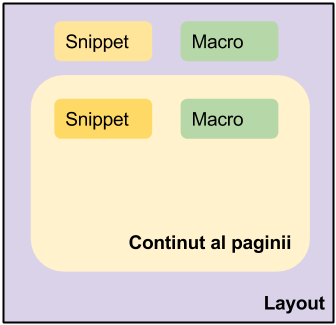
\includegraphics[scale=0.6]{roda-page.png}
\end{center}



\textbf{Layout-ul} este ansamblul de elemente HTML care nu se modifica foarte mult de la o pagina la alta si care imprima o mare parte din designul general al acesteia. De asemnea, layoutul poate contine meniuri, headere, footere si alte elemente care se mentin la trecerea de la o pagina la alta. Site-ul poate avea oricate layout-uri iar acestea pot fi modificare din interfata de administrare din sectiunea special dedicata acestora.



\bigskip

In interiorul layoutului se pozitioneaza \textbf{continutul paginii}. Acesta este de asemenea editabil din sectiunea special dedicata in itnerfata de administrare. 



\bigskip

\textbf{Snippet-ul} este un fragment de continut reutilizabil care poate fi inserat atat in layout cat si in continutul paginii. Conceput pentru fragmente de cod care se pot refolosi fie in interiorul layouturilor, fie in continutul paginilor, snippet-urile se pot adauga sau modifica in sectiunea speciala din interfata de administrare. 



\bigskip

\textbf{Macro-urile} sunt coduri speciale care determina introducerea anumitor elemente dinamice calculate de server inainte de compunerea paginii. Macro-urile sunt predefinite si pot fi utilizate in orice element de continut (layout, snippet, continutul paginii). 

\bigskip


\subsubsection*{Distributia adreselor (url dispatching)}


Distributia adreselor este operatia de transformare a unei adrese URL solicitate serverului intr-un component software care se executa si care returneaza continutul corespunzator. RODA implementeaza sistemul de controller unic pentru generarea paginilor, controller care la primirea unui URL care incepe cu /page/ va executa urmatoarele operatii:

\begin{itemize}
\item
va solicita bazei de date toate informatiile despre pagina respectiva. 
\item
va cauta layout-ul paginii respective.
\item
va executa (recursiv) toate macro-urile din layout + pagina, incluzand toate elementele solicitate de acestea.
\item
va returna pagina astfel compusa. 
\end{itemize}

\subsubsection*{Interfata de administrare}

Interfata de administrare pentru modulul CMS contine urmatoarele module:
\begin{itemize}
\item
Modulul pentru administrarea paginilor
\item
Modulul pentru administrarea snippet-urilor
\item
Modulul pentru administrarea layout-urilor
\item
Modulul pentru administrarea fisierelor statice
\end{itemize}

\bigskip

Aceste module sunt prezentate in detaliu in Anexa 1. In figura urmatoare se poate vedea aspectul interfetei de administrare al paginilor.

\begin{center}
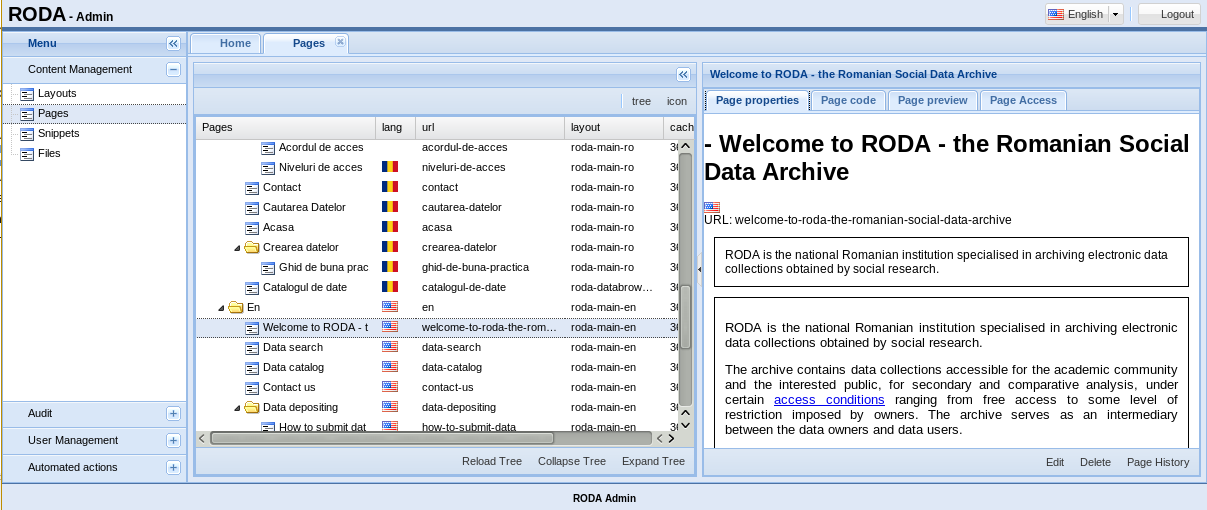
\includegraphics[width=16.1cm,height=8.1cm]{cmspages.png}
\end{center}

\subsection*{Interfata de administrare a utilizatorilior sistemului}

Modulul pentru managementul utilizatorilor este componentul interfetei de administrare care permite adaugarea, stergerea, modificarea precum si alte operatii asupra utilizatorilor sistemului RODA. Utilizatorii sunt impartiti in grupuri iar permisiunile sunt determinate de apartenenta la unul sau mai multe grupuri. 


Interfata de management de utilizatori permite urmatoarele operatii:

\begin{itemize}
\item
Afisarea listei utilizatorilor
\item
Afisarea listei grupurilor
\item
Afisarea detaliilor utilizatorilor, a mesajelor acestora
\item
Modificarea proprietatilor utilizatorilor
\item
Trimiterea mesajelor catre grupuri de utilizator

\end{itemize}


\bigskip

In anexa 1 sunt prezentate detalii despre modulul de management al utilizatorilor.



\subsection*{Interfata de administrare pentru sistemul de jurnalizare.}


Interfata de administrare pentru modulul de jurnalizare permite urmarirea tuturor modificarilor aduse de utilizatori asupra datelor aflate in baza de date. 

\bigskip

Sistemul de jurnalizare este un sistem care functioneaza automat, legat direct la sistemul de management al datelor si care inregistreaza toate modificarile facute asupra bazei de date, permitand refacerea acestora acolo unde este cazul. 



\bigskip

Pentru fiecare revizie se pot vedea toate obiectele modificate, toate randurile afectate de fiecare modificare precum si valorile anterioare modificarii curente. O imagine a acestui modul se poate vedea in figura urmatoare:

\begin{center}
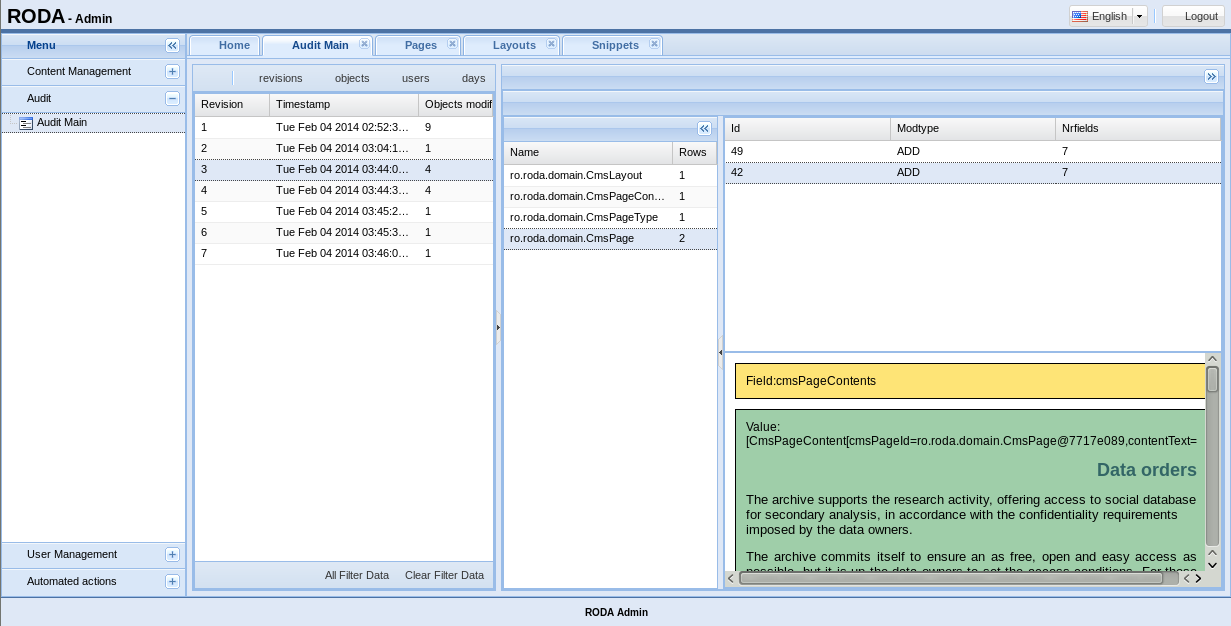
\includegraphics[width=16.1cm,height=8.1cm]{audit.png}
\end{center}


Mai multe detalii cu privire la interfata si functionarea acestui modul se afla in Anexa 1


\bigskip

\medskip

\clearpage

\section{Rezultate, stadiul realiz\u{a}rii obiectivului, concluzii si propuneri pentru continuarea proiectului}

%TODO de completat la fiecare faza ???

\medskip

Obiectivele pentru aceasta faza au fost indeplinite, fiind implementate sistemul de management de continut, utilizatori precum si al jurnalizarii. 
Implementarile sunt corecte si complete, modele de lucru cunoscute iar interfetele de management permit executia tuturor operatiilor necesare pentru o buna functionare a managementului de continut, utilizatori precum si urmarire a modificarilor datelor (jurnalizare). 

%\clearpage

\bigskip

\bigskip

\bigskip

\bigskip

\bigskip

\bigskip

\bigskip

\bigskip

{\bfseries
RECTOR,}

prof.univ.dr. Mircea Dumitru

\bigskip

\bigskip

\bigskip

\bigskip

\bigskip

\bigskip

\bigskip

\bigskip

{\bfseries
DIRECTOR GENERAL ADMINISTRATIV,}

ec. Adrian Albu

\bigskip

\bigskip

\bigskip

\bigskip

\bigskip

\bigskip

\bigskip

\bigskip

{\bfseries
RESPONSABIL PROIECT,}

lect.univ.dr. Adrian Du\c{s}a

\end{document}
